\documentclass{article}
\usepackage{graphicx}

\usepackage{amsmath}
\usepackage{wasysym}
\usepackage{graphicx}
\usepackage{caption}
\usepackage{subcaption}
\title{Methods for Parsing Dipmeter Images }
\date{August 2023}

\author{Bryan Azbill}

\begin{document}
\maketitle 
\section{Introduction}
The angle of rotation from horizontal along a layer of rock is called its dip. Wells typically pass through many layers of rock. Interests in measuring the dip of layer for such wells can be served by a device called the dipmeter, and it is common practice to store data collected with a dipmeter in a format referred to as the arrow or the tadpole plot. 
Dip logs for many wells have been stored as tadpole plots. Tadpole plots contain a cartesian grid to record each measurement over with the placement of a circle and juxtaposed perpendicular line, loosely in the shape of a tadpole, similar to a  \male . These shapes record the layers depth with their horizontal position, dip by their vertical position, 
These plots became common practice because they are convienently readable by human eyes, but when they are the only record available from a previous dip survey for a well, and those records are desired for a computational study, it is problematic to parse digital images of tadpole plots into numerical data for analysis.
These images are often scanned in poor condition, the gridlines unevenly spaced and faded, the tadpoles distorted, and the images are not only crooked wavering in their angle. Having lines superimposed over the shapes makes distinquishing them particularly difficult, like captcha images. 
Granted, the images are not as bad as the captcha,  but the problem is similar. Even though very effective algorithms for image parsing the likes of captcha systems have been already implemented with convolutional deep learning, they are not directly applicable to this problem because they rely on the fact that images are generated by a computer
enable the generation of arbitrarily large training set images with known answers. The more traditional approaches used in this study circumvent the need for training sets by using a priori knowledge of the tadpole image to manually structure kernals for convolution and other filtering operations
in order to overcome the above mentioned challenges and reliably extricate the different components superimposed in the image.  The problem is broken down as follows,

\begin{enumerate}
    \item extricating a grid from the rest of an image when
        \subitem the grid is located among other parts of the log
        \subitem the grid is not straight, even at an angle
        \subitem the grid is not perfectly spaced
        \subitem the grid fades out in places
        \subitem the grid is interspaced with other tadpoles

    \item extricating the tadpole circles placed upon the grid image when, 
        \subitem the image is distorted
        \subitem clearing the grid from the circles adds further distortion
        \subitem some circles are solid while others are not          
        \subitem resolution may be low

    \item comparing the pixel location of each tadpole to that of the gridlines to determine the depth and dip of each measurement when
        \subitem the grid is not perfectly spaced   

    \item extricating the angle of the line tailed on each tadpole, when
        \subitem clearing both the circles and gridlines from the image prevents their
        interference introduces but iintroduces further distortion
        \subitem some lines intersect other circles and gridlines   
\end{enumerate}
    
          




The tadpoles interfere with detection on the grid. The grid interferes with detection on the tadpoles. both subset only a portion of the larger log image. 
the stricter a filter must be to remove the interference, the more undesired interference there will to the structure the filter is trying to isolate, so what gives? 
It stands to reason that as more information already collected on the image, the more strategically operations can be applied. The trick is bootstrapping an 
alternation series of algorithms which filter, algorithms which restore, and  algorithms which detect.  A series to use previous detections 
for progressively balancing the next round with less selective and distorive filters, applying both filters and detection at more strategic subsets of the image.



\section{Methods}
The following order structures the application of filters, detections, and restorations to the image:
\begin{enumerate}
    \item identifying the location of the grid 
    \item restoring the image to a straightened grid
    \item identifying the line spacing of the grid
    \item identifying the locations of each tadpole
    \item identifying the angle of the line extending each tadpole
    \item converting each tadpoles pixel location to its placement relative to the cartesian grid
\end{enumerate}
    

    The filters chosen in this study are:
    \begin{itemize}
        \item[Convolutional Filters] 
        \subitem With kernals manually designed, they can be highly selective for isolating structures chosen for detection at the beginning of the process,
        before much else can be used to cleared other parts of the image or used for guidance on where to look.                                
        \subitem With kernals selected from regions of the image, they can be used to compare the rest of the image with the selected region
        \item[Morphological Erode] Is effective at clearing previously detected structures from the image with minimal distortion and is used more
        towards the end of the process.
        \item[Morphological Open]
    \end{itemize}

    The algorithms chosen for detection are:
    \begin{itemize}
        \item[Peak Detection] either applied to the image directly, or to a list of sums of the image by row or column
        \item[Hough Transform] to locate circles
        \item[Template Matching] to detect the angle on the tadpole tails 
    \end{itemize}

    The algorithms used which restore are:
    \begin{itemize}
        \item[shifting] to straighten the image                     
    \end{itemize}
    An algorithm used which both filters and restores: 
    \begin{itemize}
        \item[Threshold] applied to faded structures to remove what's too faded, and blacken what's not.
    \end{itemize}
        

    \subsection{Identifying the location and spacing of the cartesian grid}
        Identifying the grid is the first step because it is the simplest to identify.
        This is because they can be  distinguished by the fact that they are nearly vertical, horizontal, and 
        also extend across large portions of the image.

        The following kernal is used to identify vertical edges, it is called a Prewitt tranform,
        and compares to numerically computing a partial x derivative,
        \begin{gather}
            P = 
            \begin{matrix}
                1/3 & 1/3 & 1/3\\
                0 & 0 & 0\\
                -1/3 & -1/3 & -1/3
            \end{matrix}
        \end{gather}
        To be used on horizontal lines, it simply needs be transposed  
        For lines, however, it is better to compute the second partial derivative, 
        which is done by applying the prewitt transform twice. Finally the line filter should favor lines that continue for some distance.
        To accomplish this, the image is horizontally blurred with one final 1xn matrix with elements uniformly as 1/n, 
        where n defines the blur distance. I call it $B_n$ . all together, a kernal $L_h$ is computed to be

        \begin{equation}
            L_h= P \ast P \ast B_n
        \end{equation}

        where * denotes a convolution product.

        From $L_h$, a vertical line convolution filter can be constructed trivially by simply computing the transpose of $L_h$,
        \begin{equation}
            L_v = L_h^t
        \end{equation}

        To further clarify the lines after applying these filters, it helps to process with a threshold transformation. Then the results are very effective.
        Consider the following images as examples,

        \begin{figure}
            \centering
            \begin{subfigure}{.3\textwidth}
                \centering
              
              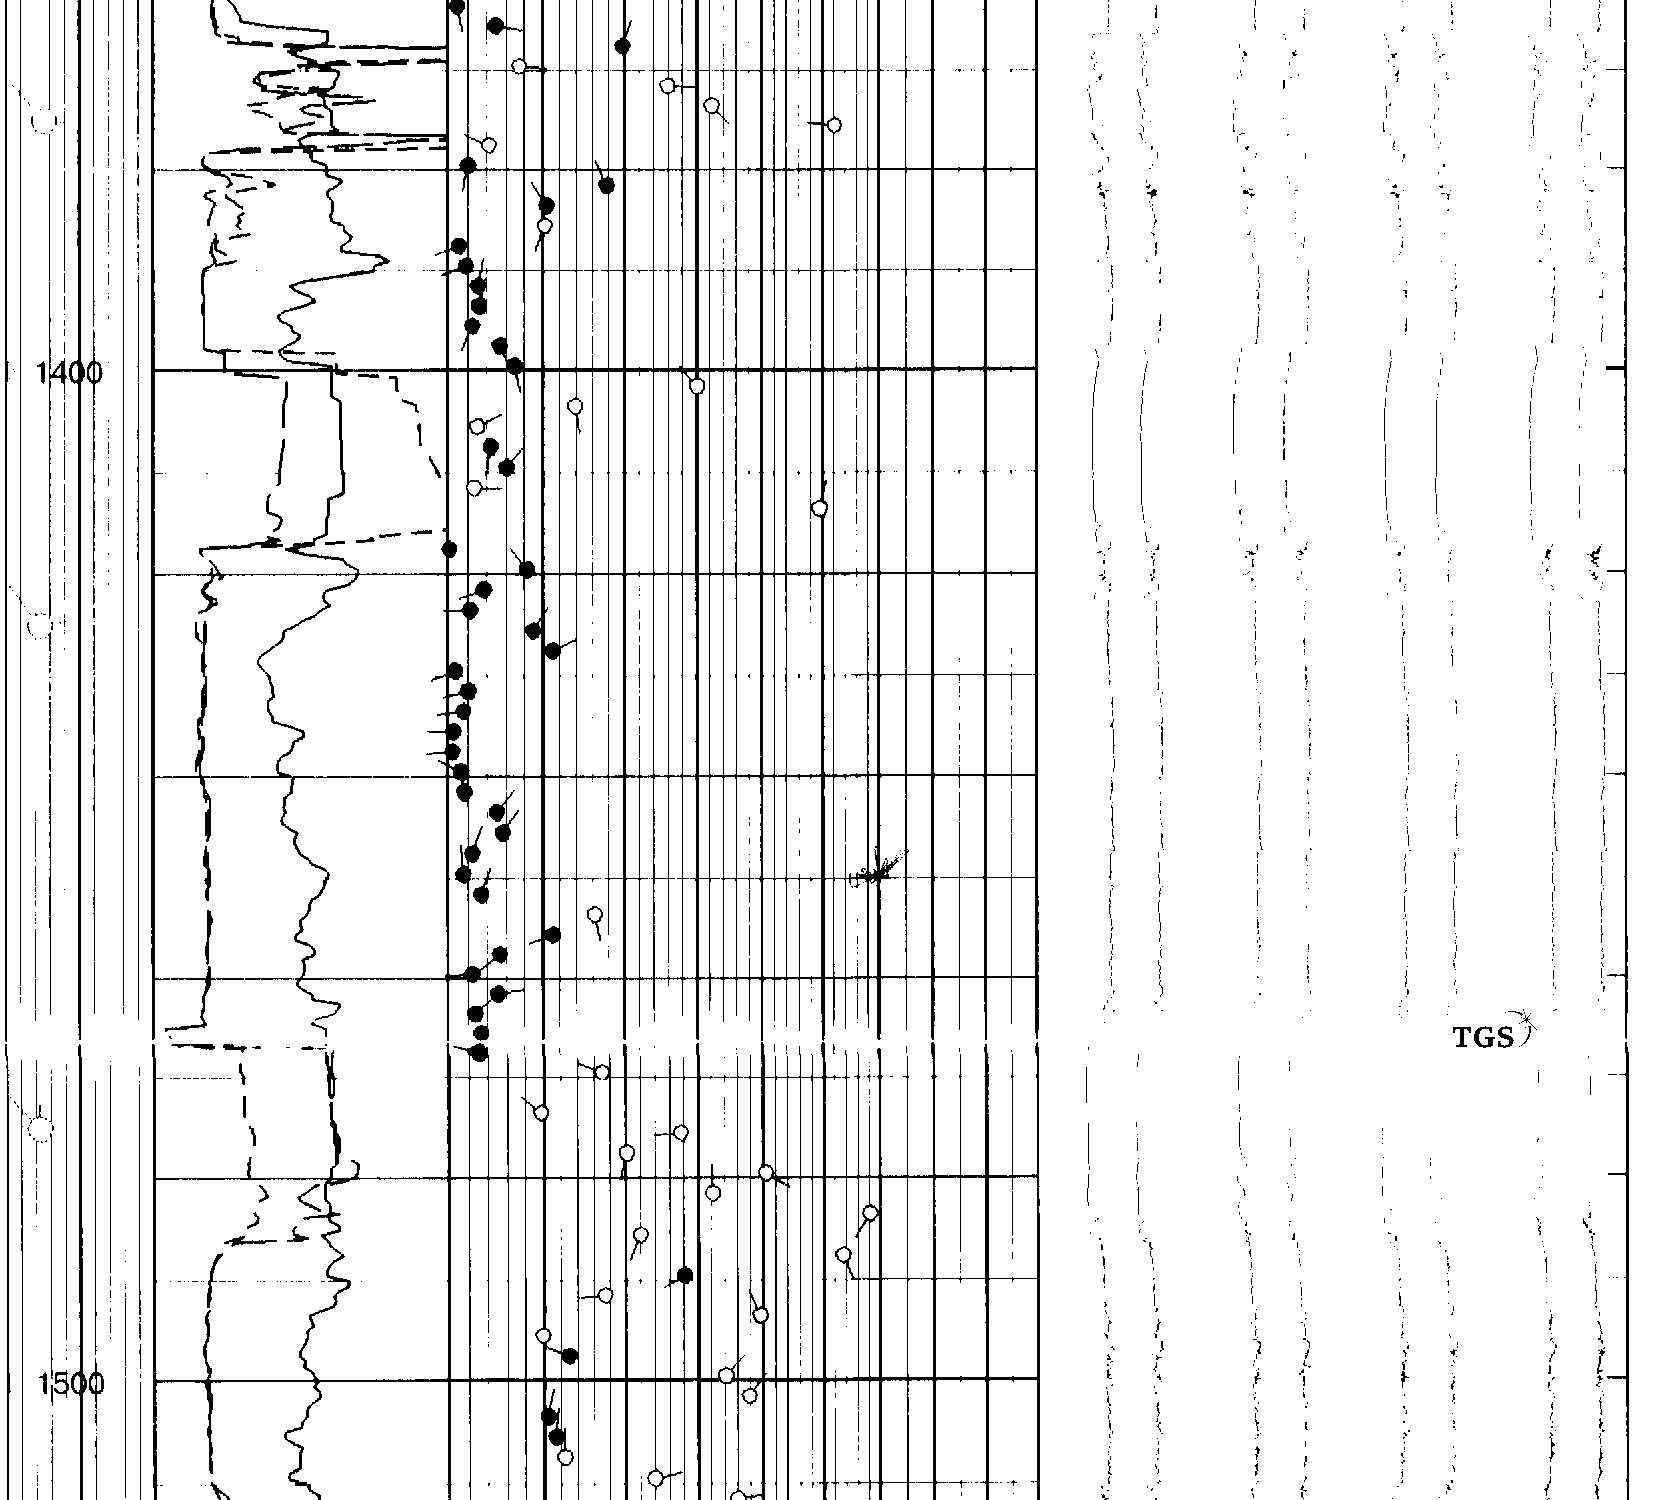
\includegraphics[width=\textwidth]{figures/unfiltered.jpg}
              \caption{Original}
              \label{fig:unfiltered}
            \end{subfigure}
            \hfill
            \begin{subfigure}{.3\textwidth}
                \centering
                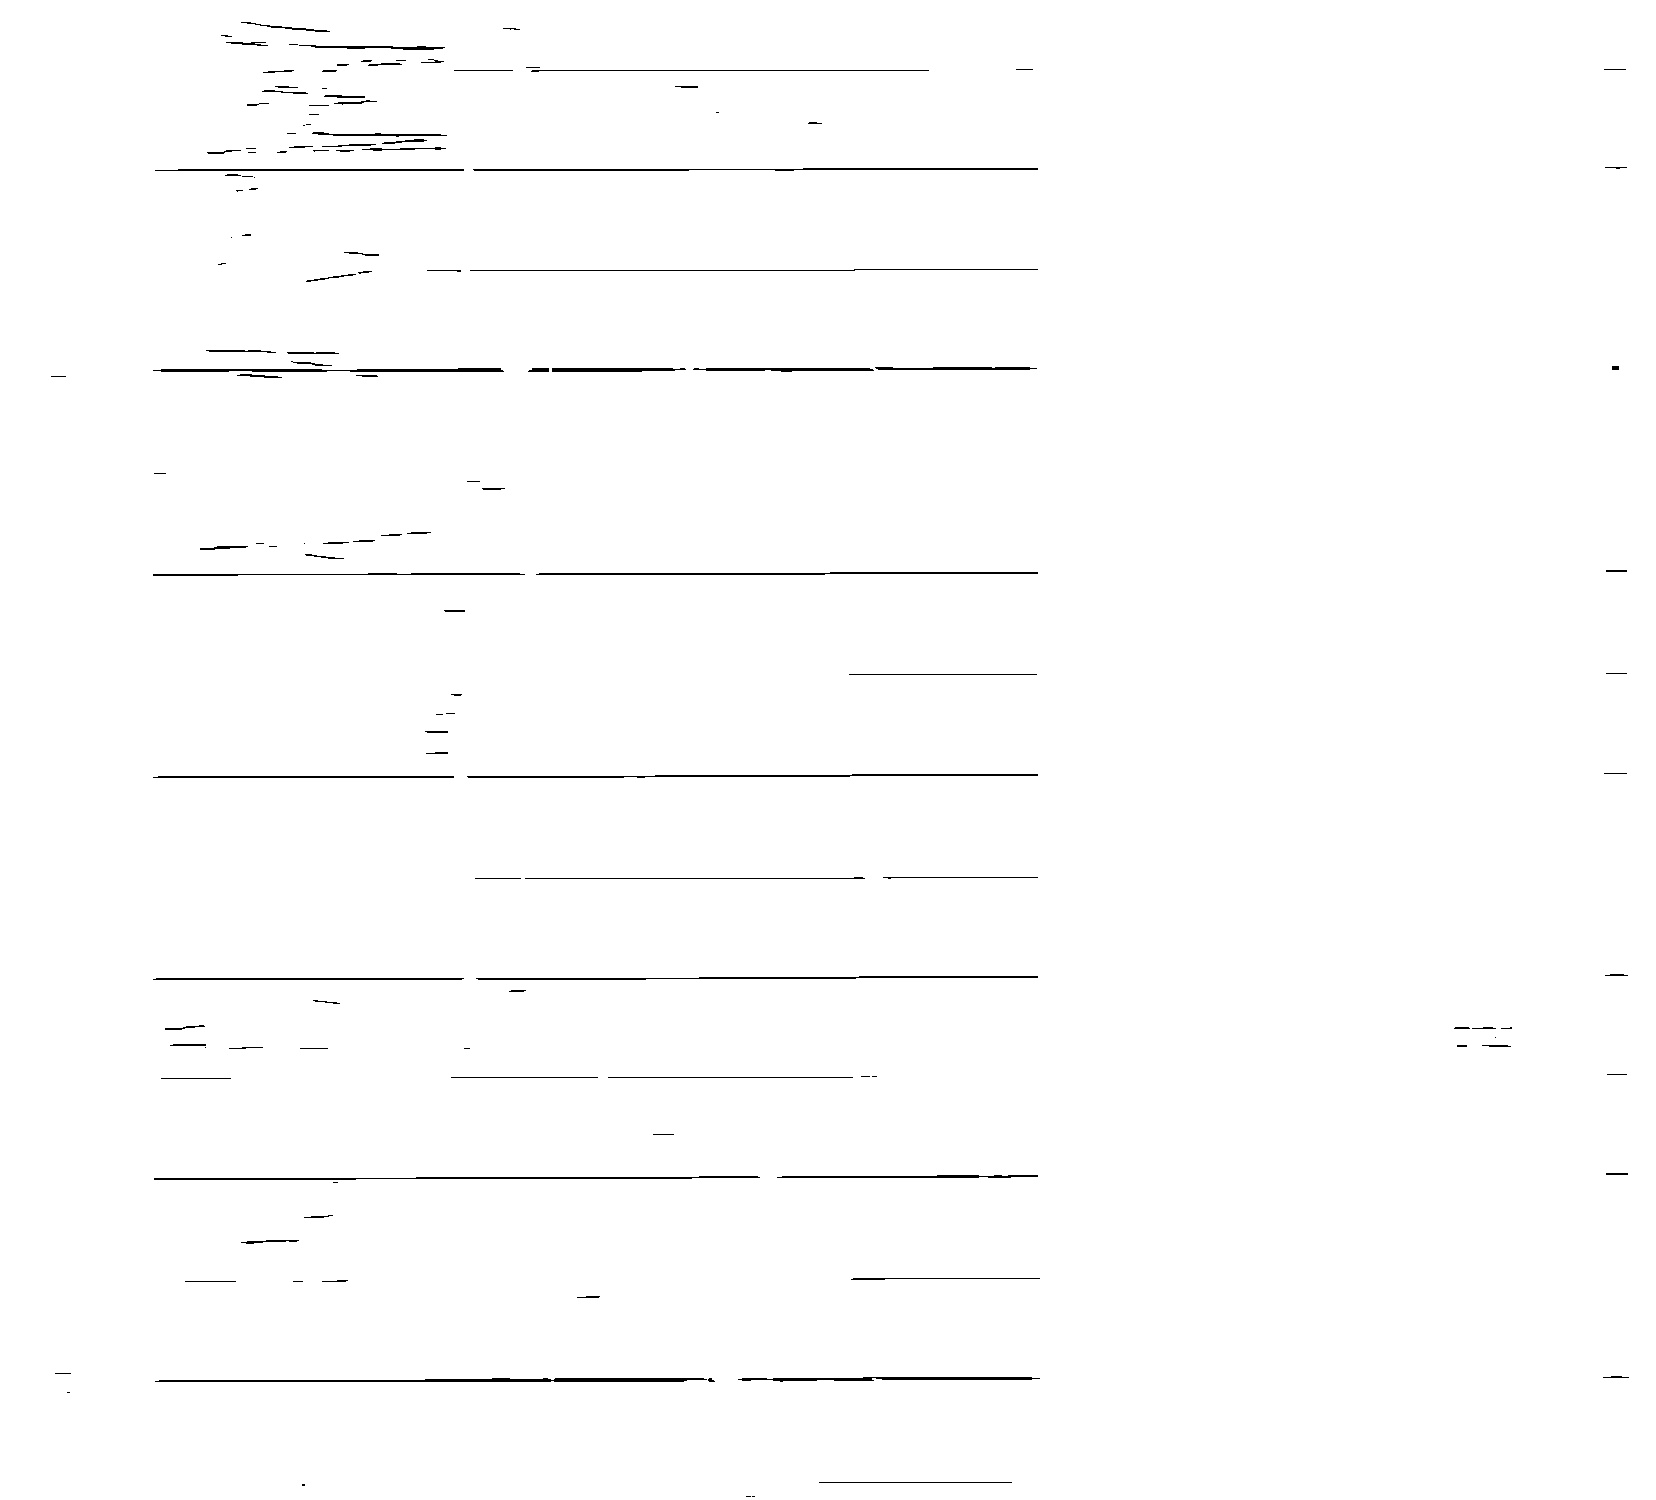
\includegraphics[width=\textwidth]{figures/hFilter.jpg}
              \caption{With $L_h$}
              \label{fig:hFilter}
            \end{subfigure}
            \hfill
            \begin{subfigure}{.3\textwidth}  
                \centering              
                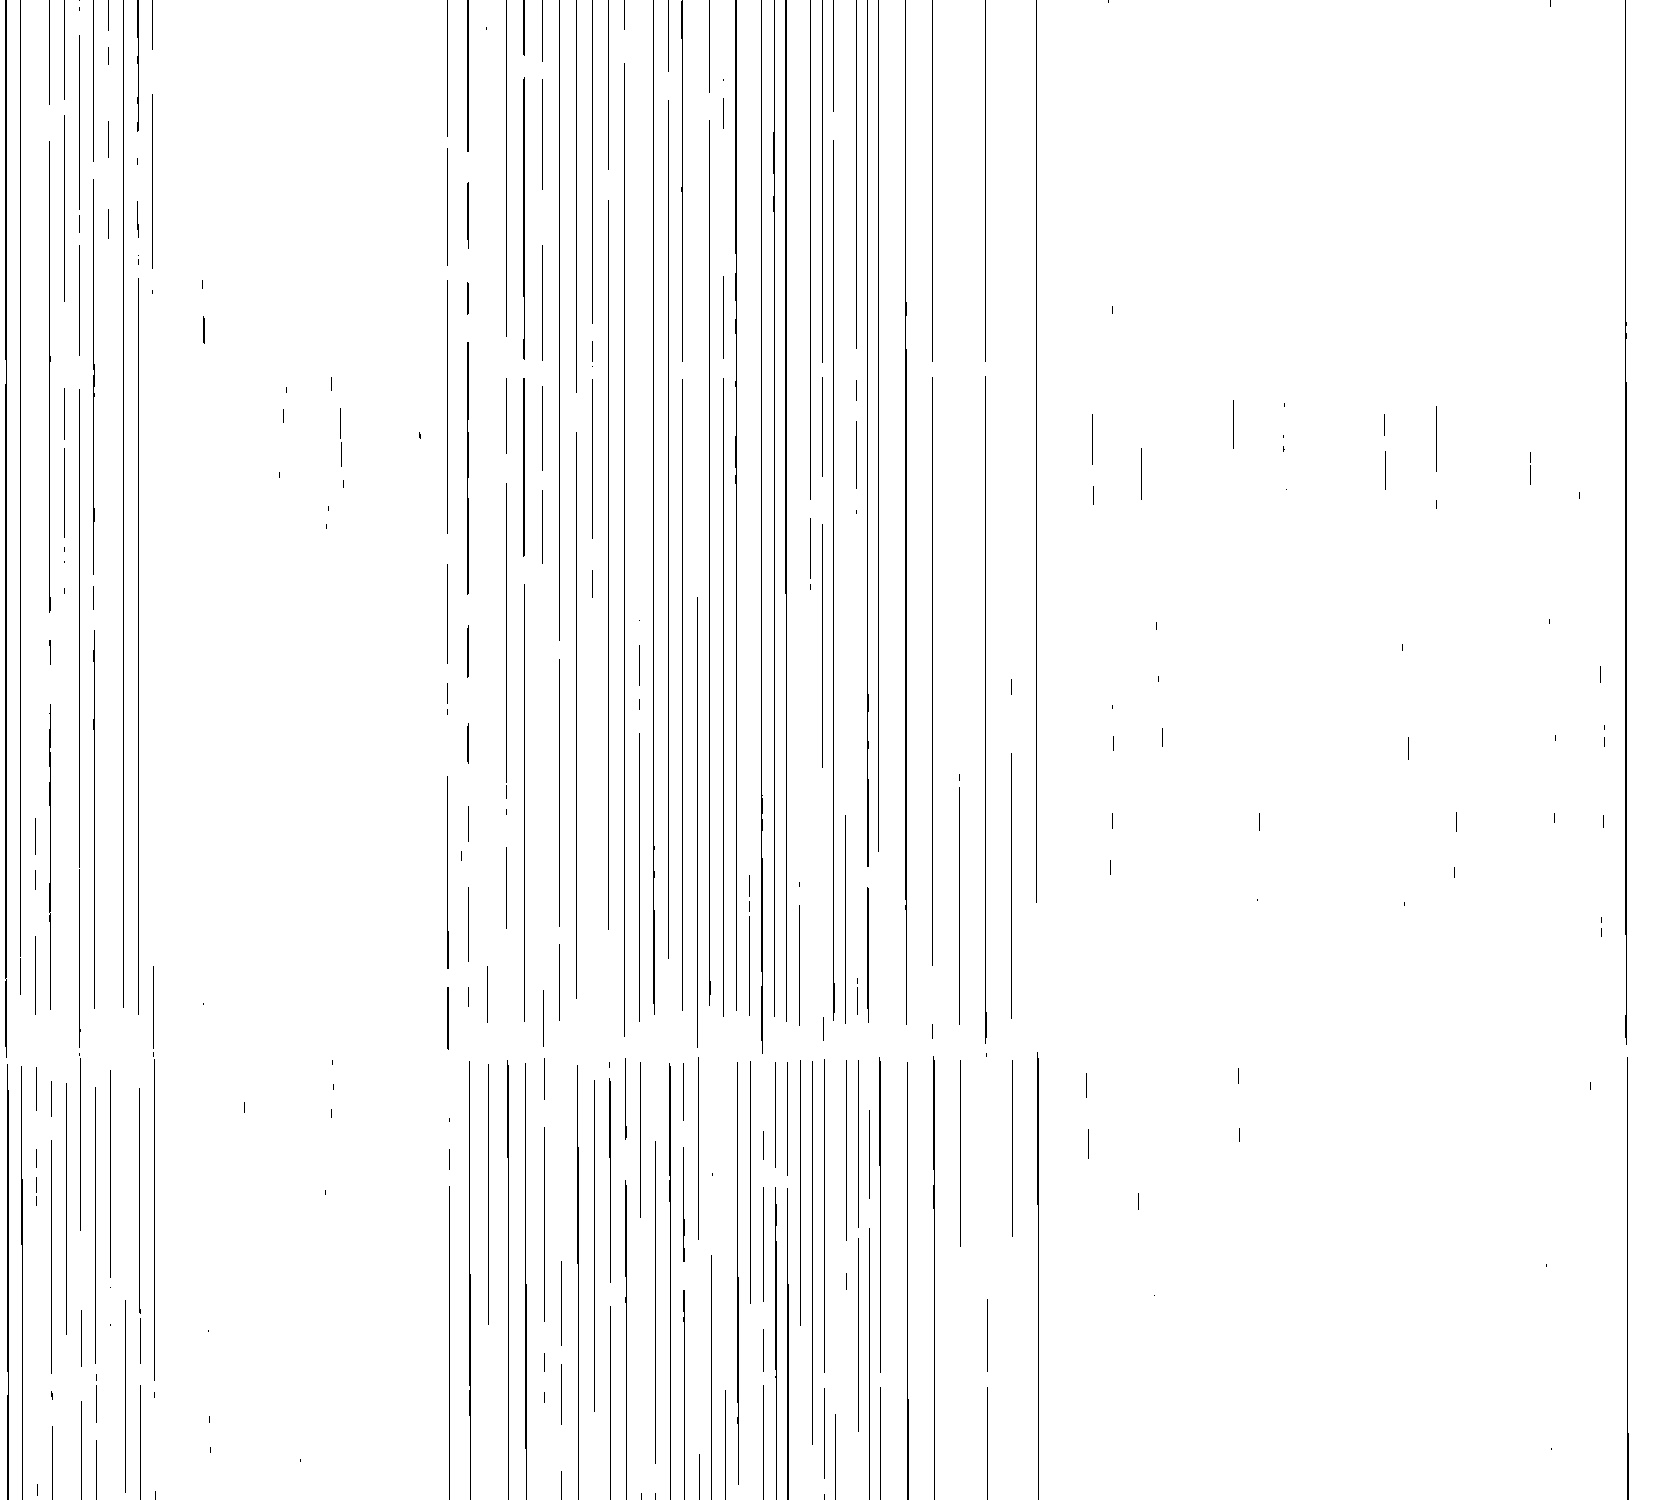
\includegraphics[width=\textwidth]{figures/vFilter.jpg}
                \caption{With $L_v$}
                \label{fig:vFilter}
            \end{subfigure}
            figures\
            \caption{Filtering Out Lines}
            \label{fig:Convolutional Line Filtering}
        \end{figure}
        With the image filtered for lines, it is possible to identify the region between the top, bottom, left, and of the grid. by summing the filtered images row and column to find the peak where the lines are dense.
    
    \subsection{Straightening the Image and Detecting the Grid}
        Once the gridlines are detected, they can be used to detect shift in the image. 
        Using the top of the grid filtered vertically as the kernal template for filtering the whole image, a convolution product is computed which reveals how the rows below can be shifted for 
        their lines to match the top of the kernal. In a similar process, the column shifts are likewise identified.     
        once this distortion is identified, it can be corrected by shifting the image.

    \subsection{Detecting The Tadpole Circles}
            When it comes to identifying the circles in an image, the Hough Transform is a standard and effective algorithm. However, it cannot be applied directly to the image, because the gridlines will interfere with the detection.
            Therefore the gridlines must be cleared from the straightened image. Simply coloring them white distorts the circles. This is where morphological operations are useful. The morphological erode operation can be structured to 
            whiten out the boundaries of every shape a chosen distance in either the vertical or horizontal direction. Such a distance can be chosen to be just enough to erase a whole gridline. Then, the morphological open operation is applied to 
            invert the erosion, restoring any shape so long as it was not completely erased during the erosion. The combination of these two operations is called a morphological close, and is very effective at clearing the lines from the image
            while leaving minimal distortion to the circles. Additionally, the operation is only applied to the regions around each gridline. 
            The following image shows the result of applying the morphological close operation in such a manner
            \begin{figure}
                \centering
                \begin{subfigure}{.4\textwidth}
                    \centering                  
                  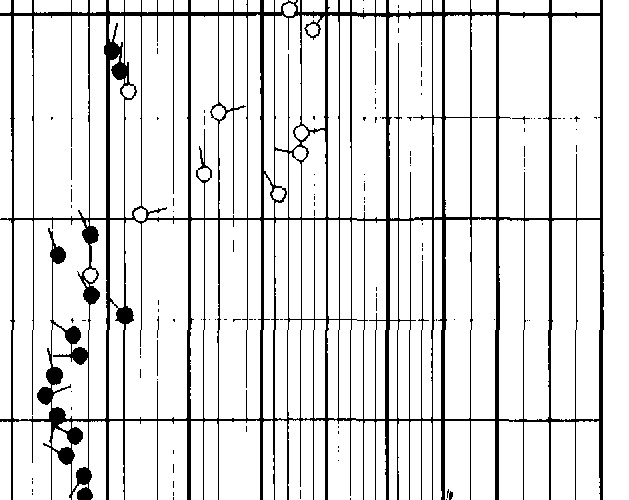
\includegraphics[width=\textwidth]{figures/straight3ex.jpg}
                  \caption{a cut of the straightened image before clearing}
                  \label{fig:straight}                
                \end{subfigure}
                \begin{subfigure}{.4\textwidth}
                    \centering
                    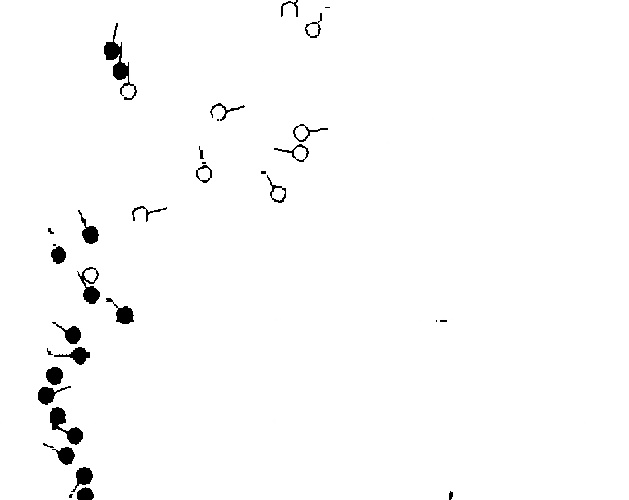
\includegraphics[width=\textwidth]{figures/noGrid.jpg}
                  \caption{a cut of the straightened image after clearing}
                  \label{fig:no_grid}
                \end{subfigure}                                 
                \caption{Filtering Out Lines}   
            \end{figure}
            

            Without nothing else to interfere, param Hough Transform can be applied to the image to detect where the tadpoles are placed with high sensitivity. In the first round of detection however some circles can be missed. 
            Therefore, the first circles to be detected are erased from the image by simply drawing them white, and then the Hough Transform is applied again to detect the remaining circles. The following image shows the result of this process.
            \begin{figure}
                \centering
                \begin{subfigure}{.3\textwidth}
                    \centering                  
                  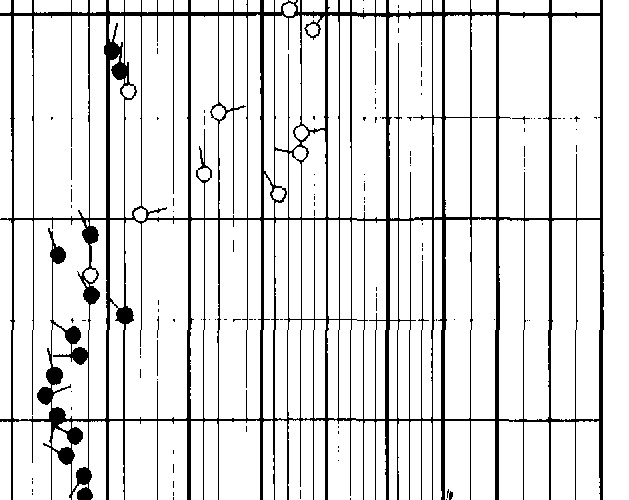
\includegraphics[width=\textwidth]{figures/straight3ex.jpg}
                  \caption{Original}
                  \label{fig:straight}
                \end{subfigure}
                \hfill
                \begin{subfigure}{.3\textwidth}
                    \centering
                    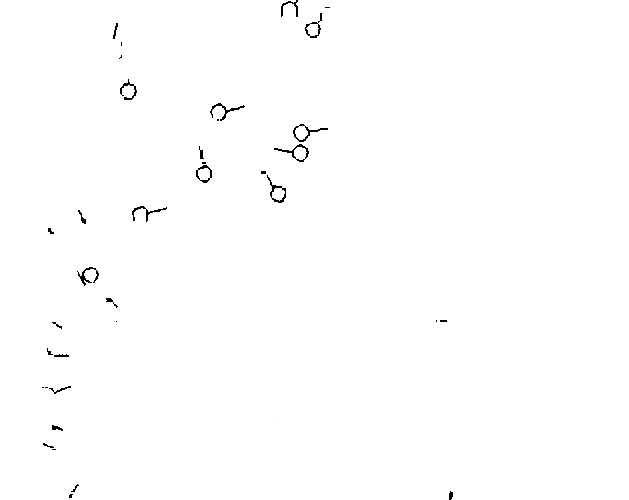
\includegraphics[width=\textwidth]{figures/noCirc2.jpg}
                  \caption{With First detections removed}
                  \label{fig:noCirc}
                \end{subfigure}
                \hfill
                \begin{subfigure}{.3\textwidth}  
                    \centering              
                    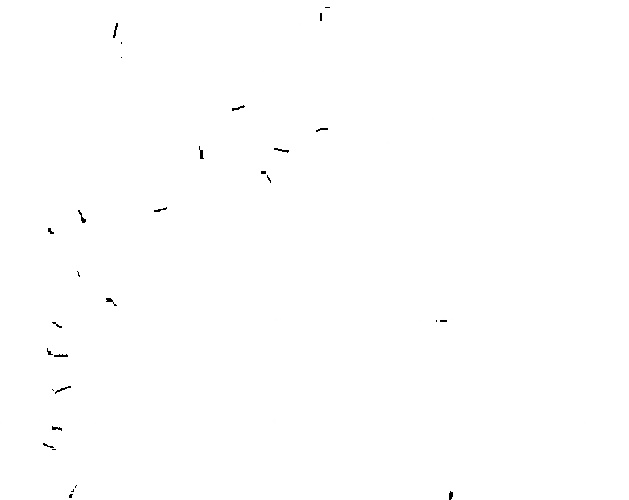
\includegraphics[width=\textwidth]{figures/noCirc3.jpg}
                    \caption{With Second detections removed}
                    \label{fig:noCirc2}
                \end{subfigure}
    
                \caption{Filtering Out Lines}
                \label{fig:test} 
            \end{figure}
        
        \subsection{Processing the Tadpoles}
            In order for the tadpoles to be accurately identified, its necessary to mask out the underlying grid, so as not to confuse the gridlines with tadpoles. Once only the tadpoles remain with image, running a Hough transform algorithm out of a package is very effective in locating each circle, 
            as well as computing their radius. 
            Some tadpole circles are filled, while others are not. It's simple enough just to add up some of the pixels in the middle to determine the case for each one. Then it needs to be double checked if its really a circle. Doing this can be simply done by drawing another circle over the top 
            and checking the difference. Once a tadpole is confirmed, the angle of the line extending from it needs to be determined. It is easy to do this by masking the circle from the tadpole and then using another out of the package algorithm. In some cases, however, the tadpole line is overlapped
            with a gridline, and so gets masked with the gridline. Therefore, lines with a poor match should be listed, so that at least the user of the script can identify 

        \section{results}
         to be continued
        \section{Conclusion}

            The algorithms for this project were tested in python, which can be rather slow. Algorithms were tested from two libraries, OpenCV and Scikit-image. The OpenCV algorithms are compiled in C and just wrapped in python, and so therefore run very fast. 
            Convolutions,  hough transforms, and morphological operations where all best processed with OpenCV. Scikit-image is typically much slower, because it is not compiled in C. Scikit-image, however, is often easier to use and has a more comprehensive collection of tools with it. It's rather impressive. However,
            even after a great deal of time spent exploring the package and running tests with them, none provided better accuracy than effectively using the classic algorithms in OpenCV.
            Nonetheless, I found that often, major downsampling the image first can be done to improve runtime without compromising tests, and even though OpenCV bears the load of my final  ideas for convolution kernal design that were key to finally cracking the whole problem were inspired by my study and experimentation with scikit-image.
    \end{document}